
%(BEGIN_QUESTION)
% Copyright 2007, Tony R. Kuphaldt, released under the Creative Commons Attribution License (v 1.0)
% This means you may do almost anything with this work of mine, so long as you give me proper credit

The EIA/TIA-232 digital communications standard (formerly known as RS-232) is an early standard for serial communication still in use today.  The standard ``pinout'' for a 9-pin D-subminiature connector looks like this.  This form of connector is properly known as a DE-9, but is commonly (and erroneously) referred to as a DB-9:

$$\includegraphics[width=15.5cm]{i02189x01.eps}$$

When used on a digital device that generates or interprets serial data (such as a computer), called a {\it DTE} (Data Terminal Equipment), the pin assignments are as follows (essential pins labeled in {\bf bold}):

\begin{itemize}
\item{} Pin 1 = Carrier Detect (CD)
\vskip 5pt 
\item{} Pin {\bf 2} = {\bf Received Data} (RD)
\vskip 5pt 
\item{} Pin {\bf 3} = {\bf Transmitted Data} (TD)
\vskip 5pt 
\item{} Pin 4 = Data Terminal Ready (DTR)
\vskip 5pt 
\item{} Pin {\bf 5} = {\bf Signal Ground}
\vskip 5pt 
\item{} Pin 6 = Data Set Ready (DSR)
\vskip 5pt 
\item{} Pin 7 = Request To Send (RTS)
\vskip 5pt 
\item{} Pin 8 = Clear To Send (CTS)
\vskip 5pt 
\item{} Pin 9 = Ring Indicator (RI)
\end{itemize}

When used on a device that merely passes serial data on through a network (such as a modem), called a {\it DCE} (Data Communication Equipment), the assignments of pins 2 and 3 are swapped.  For a DCE, pin 2 is for transmitting data (to a DTE device) and pin 3 is for receiving data (from a DTE device).  This way, a ``straight-through'' cable connecting pins 2 to pin 2, pin 3 to pin 3, and pin 5 to pin 5 is all that is needed for a DTE (computer) to talk with a DCE (modem).

\vskip 10pt

Explain the purpose of these pin assignments.  In the regular cycle of serial communication between two EIA/TIA-232 devices, what roles do these lines play, if any?

\vskip 20pt \vbox{\hrule \hbox{\strut \vrule{} {\bf Suggestions for Socratic discussion} \vrule} \hrule}

\begin{itemize}
\item{} Explain the purpose of {\it flow control} in a serial data network.
\end{itemize}

\underbar{file i02189}
%(END_QUESTION)





%(BEGIN_ANSWER)

Most of these lines have to do with {\it handshaking}, while only the TD, RD, and Ground lines are absolutely essential to communication.  As it turns out, handshaking may be achieved through the use of signals on the TD and RD lines instead of the dedicated handshaking lines.  This is called {\it software handshaking}, and it is more popular than hardware handshaking in modern EIA/TIA-232 systems.  The following illustration shows data flow direction along these conductors (i.e. which device transmits and which device receives):

$$\includegraphics[width=15.5cm]{i02189x02.eps}$$

\vskip 10pt

Software handshaking -- particularly the XON/XOFF standard -- has its origin in early printer devices, which could not print as fast as computers could send them information.  These printers had RAM memory buffers for holding data prior to printing, but these were too small to store the entire print job, and so would fill up before the printing was done and before the entire job could be sent.  Printers needed a way to tell their sending computers to halt transmission of data (XOFF) so that the buffer could empty, and to re-establish transmission (XON) when the buffer was sufficiently empty.  

Command-line user terminals in UNIX systems adopted the keybindings $<$Ctrl$>$ $<$S$>$ for XOFF and $<$Ctrl$>$ $<$Q$>$ for XON, so that users could halt and re-establish the transmission of a long text stream at will.

\vskip 10pt

Apparently, a true DB-9 connector (not a {\it DE-9}) has the same shell as the DB-25, but with only 9 pins in it!  The smaller shell has its own unique letter designation, which is DE- instead of DB-.

%(END_ANSWER)





%(BEGIN_NOTES)


%INDEX% Networking, serial: EIA/TIA-232 (formerly RS-232)

%(END_NOTES)


